\chapter{Lab 6 - Operational Amplifiers Applications}

%%%%%%%%%%%%%%%%%%%%%%%%%%%%%%%%%%%%%%%%%%%%%%%%%%%%%%%%%%%%%%%%%%%%%%%%%%%%%%%%%%%%%%%%%%%%%%%%%%%%%%%
\section{Objective}
%%%%%%%%%%%%%%%%%%%%%%%%%%%%%%%%%%%%%%%%%%%%%%%%%%%%%%%%%%%%%%%%%%%%%%%%%%%%%%%%%%%%%%%%%%%%%%%%%%%%%%%

The purpose of this lab is to delve in to the applications of operational amplifiers. There is an almost endless number of applications, the possibilities are often not intuitively obvious for students seeing them for the first time. 

%%%%%%%%%%%%%%%%%%%%%%%%%%%%%%%%%%%%%%%%%%%%%%%%%%%%%%%%%%%%%%%%%%%%%%%%%%%%%%%%%%%%%%%%%%%%%%%%%%%%%%%
\section{Materials}
%%%%%%%%%%%%%%%%%%%%%%%%%%%%%%%%%%%%%%%%%%%%%%%%%%%%%%%%%%%%%%%%%%%%%%%%%%%%%%%%%%%%%%%%%%%%%%%%%%%%%%%

\begin{itemize}
	\item Laptop with LTSpice
	\item Analog Discovery
	\item Breadboard
	\item Wiring kit
	\item Lab parts kit with TLV272 
\end{itemize}

%%%%%%%%%%%%%%%%%%%%%%%%%%%%%%%%%%%%%%%%%%%%%%%%%%%%%%%%%%%%%%%%%%%%%%%%%%%%%%%%%%%%%%%%%%%%%%%%%%%%%%%
\section{Introduction}
%%%%%%%%%%%%%%%%%%%%%%%%%%%%%%%%%%%%%%%%%%%%%%%%%%%%%%%%%%%%%%%%%%%%%%%%%%%%%%%%%%%%%%%%%%%%%%%%%%%%%%%

There are a variety of configurations op amps can be considered standard and while the simple inverting and non-inverting cases were show in Lab 5, here the pool is expanded to include a summing amplifier and a difference amplifier.

\begin{figure} [h!]
	\centering
		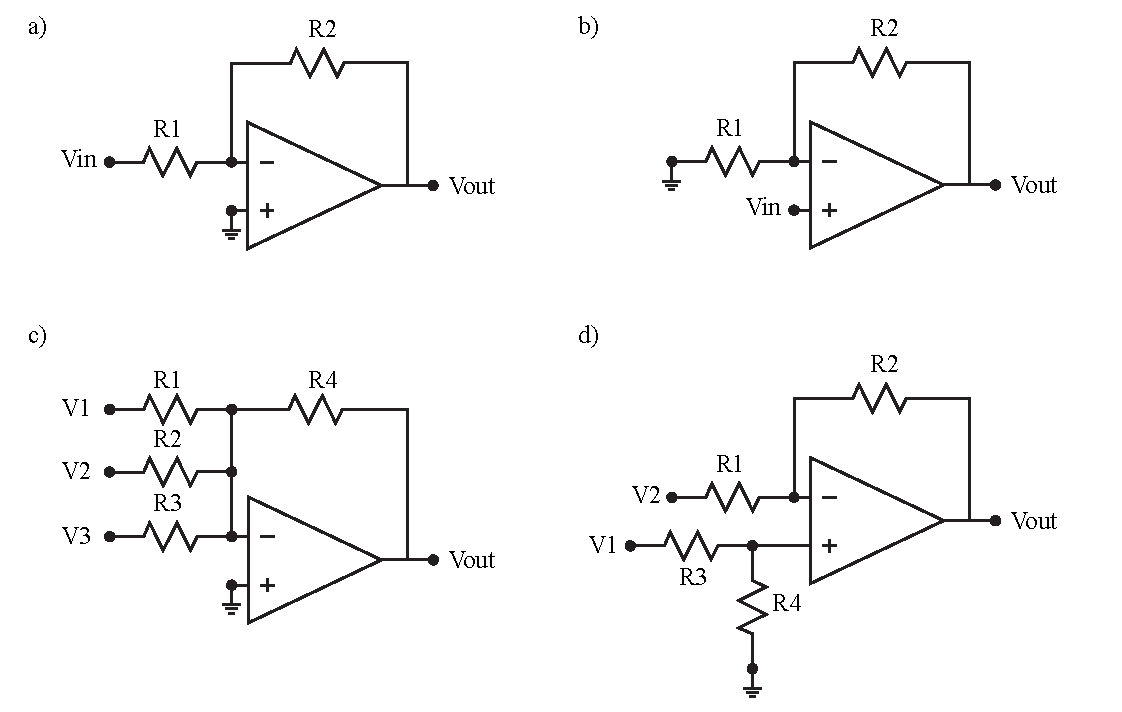
\includegraphics[width=1\textwidth]{Lab6configs.pdf}
	\caption{Different op amp configurations: inverting amplifier (a), non-inverting amplifier (b), summing amplifier (c), and difference amplifier (d).} \label{fig:6OAconfigs}
\end{figure}

%%%%%%%%%%%%%%%%%%%%%%%%%%%%%%%%%%%%%%%%%%%%%%%%%%%%%%%%%%%%%%%%%%%%%%%%%%%%%%%%%%%%%%%%%%%%%%%%%%%%%%
\subsubsection{Summing Amplifier}
%%%%%%%%%%%%%%%%%%%%%%%%%%%%%%%%%%%%%%%%%%%%%%%%%%%%%%%%%%%%%%%%%%%%%%%%%%%%%%%%%%%%%%%%%%%%%%%%%%%%%%

A summing amplifier, \hyperref[fig:6OAconfigs]{Figure \ref*{fig:6OAconfigs} (c)}, is effectively the same configuration as an inverting amplifier but has multiple inputs that allow for a weighted output voltage. 

\begin{equation}
	\centering
	V_{out} = -(\frac{R_4}{R_1}V_1 + \frac{R_4}{R_2}V_2 + \frac{R_4}{R_3}V_3)
\end{equation}

\noindent When the resistors $R_1$, $R_2$, $R_3$, and $R_4$ are all equal, the output voltage is an equal combination of the input voltages but the resistors can be chosen to weight the input voltages different based on the application. 


%%%%%%%%%%%%%%%%%%%%%%%%%%%%%%%%%%%%%%%%%%%%%%%%%%%%%%%%%%%%%%%%%%%%%%%%%%%%%%%%%%%%%%%%%%%%%%%%%%%%%%
\subsubsection{Difference Amplifier}
%%%%%%%%%%%%%%%%%%%%%%%%%%%%%%%%%%%%%%%%%%%%%%%%%%%%%%%%%%%%%%%%%%%%%%%%%%%%%%%%%%%%%%%%%%%%%%%%%%%%%%

Difference amplifiers, \hyperref[fig:6OAconfigs]{Figure \ref*{fig:6OAconfigs} (d)}, as the name implies takes the difference between the two input voltages resulting in that depends on the ratios of resistor values.

\begin{equation}
	\centering
	V_{out} =  V_1 \left(\frac{R_2}{R_1+R_2}\right)\left(\frac{R_3+R_4}{R_3}\right)-V_2\frac{R_4}{R_3}  
\end{equation}

\noindent When the resistors $R_1 = R_3$ and $R_2 = R_4$ the output voltage simplifies to 

\begin{equation}
	\centering
	V_{out} =  (V_1-V_2)\frac{R_2}{R_1}  
\end{equation}

%%%%%%%%%%%%%%%%%%%%%%%%%%%%%%%%%%%%%%%%%%%%%%%%%%%%%%%%%%%%%%%%%%%%%%%%%%%%%%%%%%%%%%%%%%%%%%%%%%%%%%%
\section{Big Picture}
%%%%%%%%%%%%%%%%%%%%%%%%%%%%%%%%%%%%%%%%%%%%%%%%%%%%%%%%%%%%%%%%%%%%%%%%%%%%%%%%%%%%%%%%%%%%%%%%%%%%%%%

\begin{figure} [h]
	\centering
		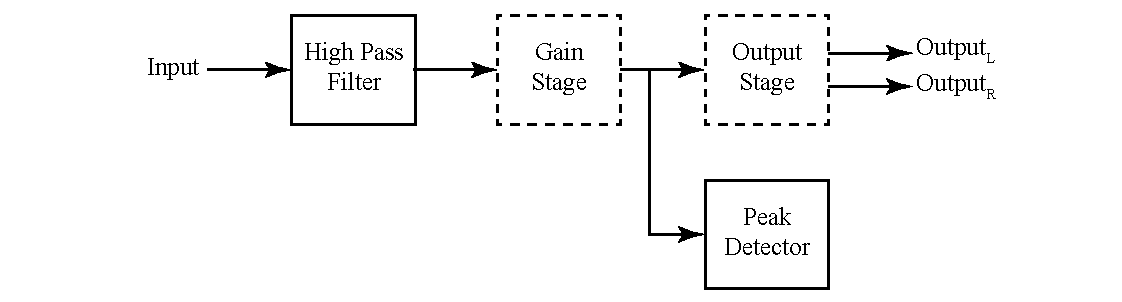
\includegraphics[width=1\textwidth]{Lab5bigpicture.pdf}
	\caption{Big picture with emphasis on the gain and output stages.} \label{fig:6bp}
\end{figure}

This lab again focuses on op amps but op amps used as different building blocks to compose more complicated circuits. The final project circuit is about as complicated as the final circuit in this lab. 

%%%%%%%%%%%%%%%%%%%%%%%%%%%%%%%%%%%%%%%%%%%%%%%%%%%%%%%%%%%%%%%%%%%%%%%%%%%%%%%%%%%%%%%%%%%%%%%%%%%%%%%
\section{Pre-Lab Requirements}
%%%%%%%%%%%%%%%%%%%%%%%%%%%%%%%%%%%%%%%%%%%%%%%%%%%%%%%%%%%%%%%%%%%%%%%%%%%%%%%%%%%%%%%%%%%%%%%%%%%%%%%

Complete the following before coming to lab. 

%%%%%%%%%%%%%%%%%%%%%%%%%%%%%%%%%%%%%%%%%%%%%%%%%%%%%%%%%%%%%%%%%%%%%%%%%%%%%%%%%%%%%%%%%%%%%%%%%%%%%%%
\subsection{Buffering} \label{ssec:6buff}
%%%%%%%%%%%%%%%%%%%%%%%%%%%%%%%%%%%%%%%%%%%%%%%%%%%%%%%%%%%%%%%%%%%%%%%%%%%%%%%%%%%%%%%%%%%%%%%%%%%%%%%

Buffering is an important op amp application because it solves a problem, loading effects, that can't easily be solved with purely resistive circuits. 

\begin{figure} [h]
	\centering
		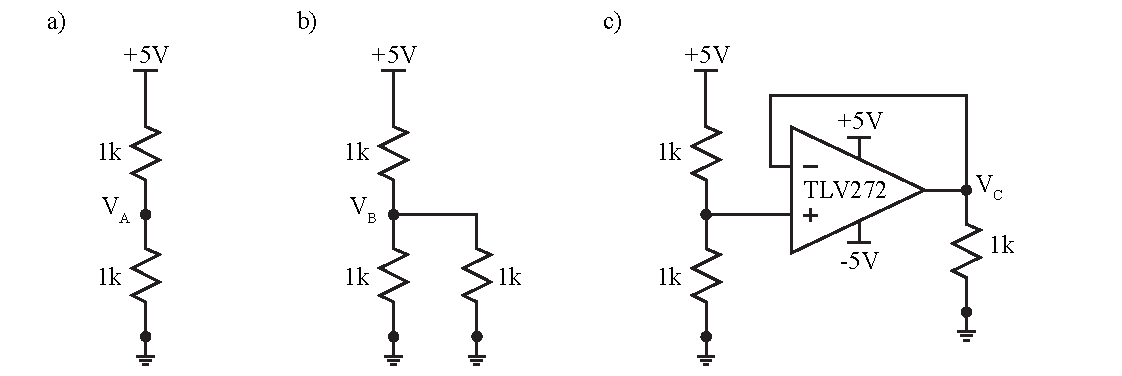
\includegraphics[width=1\textwidth]{Lab6buffering.pdf}
	\caption{A simple voltage divider (a), voltage divider with a load (b), and a voltage divider with a voltage follower between the output and the load (c).} \label{fig:6buff}
\end{figure}

\begin{enumerate}
	\item Simulate  all three circuits in \hyperref[fig:6buff]{Figure \ref*{fig:6buff}} using a DC operating point (.op). Keep all the circuits on the same schematic and table the voltages $V_A$, $V_B$, and $V_C$. Save an image of the circuit and submit the image and table in a document to Canvas. \label{itm:6ssec1itm1}
	\item Discuss why two of the voltages are approximately 2.5 V but one is not. Submit your answer as part of the document submitted to Canvas. \label{itm:6ssec1itm2}
\end{enumerate}

%%%%%%%%%%%%%%%%%%%%%%%%%%%%%%%%%%%%%%%%%%%%%%%%%%%%%%%%%%%%%%%%%%%%%%%%%%%%%%%%%%%%%%%%%%%%%%%%%%%%%%%
\subsection{Level Shifting} \label{ssec:6lvlshift}
%%%%%%%%%%%%%%%%%%%%%%%%%%%%%%%%%%%%%%%%%%%%%%%%%%%%%%%%%%%%%%%%%%%%%%%%%%%%%%%%%%%%%%%%%%%%%%%%%%%%%%%

Level shifting in electronic circuits is the process of change the supply rails from one range to another. For example, when preparing a signal for analog to digital conversion, the signal may be bi-polar (+/-) and must be converted to a single voltage rail. So, instead of a sine wave that swings to +2.5V and -2.5V, 2.5V is added so that the sine wave swings from +5V to 0V with the same amplitude. 

\begin{figure} [h]
	\centering
		\includegraphics[width=1\textwidth]{Lab6levelshift.pdf}
	\caption{A summing amplifier used to add 2.5V to $-V_{IN}$ (a) and the same configuration where the -2.5V source has been replaced with a buffered voltage divider (b).} \label{fig:6levelshift}
\end{figure}

\begin{enumerate}
	\item Simulate the circuit in \hyperref[fig:6levelshift]{Figure \ref*{fig:6levelshift} (a)} using a transient analysis with a stop time of 1m (.tran 1m). Set $V_{S}$ to a sine wave with a 0 V DC offset, 2 V amplitude, and a 1 kHz frequency. Save an image of the circuit and a plot of the input and output voltage for submission to Canvas. \label{itm:6ssec2itm1}
	\item Explain why the resistor divider in \hyperref[fig:6levelshift]{Figure \ref*{fig:6levelshift} (b)} uses -5V instead of 5V. Submit your answer as part of the document submitted to Canvas. \label{itm:6ssec2itm2}
	\item Practically, a 2.5V reference may not be available for use and instead must be self generated. Simulate the circuit in \hyperref[fig:6levelshift]{Figure \ref*{fig:6levelshift} (b)} using a transient analysis with a stop time of 1m (.tran 1m). Set $V_{S}$ to a sine wave with a 0 V DC offset, 2 V amplitude, and a 1 kHz frequency. Save an image of the circuit and a plot of the input and output voltage for submission to Canvas. \label{itm:6ssec2itm3}
	\item Construct the circuit in \hyperref[fig:6levelshift]{Figure \ref*{fig:6levelshift} (b)} on a breadboard. Configure the Wavegen to generate a sine wave at 1 kHz with a 2 amplitude and a 0V offset. Plot the input and output on the Scope and save the circuit to demo at the start of lab. \label{itm:6ssec2itm4}
	\item In the more general case, the full range of input must be accounted for. Simulate the circuit in \hyperref[fig:6fullshift]{Figure \ref*{fig:6fullshift}} using a transient analysis with a stop time of 1m (.tran 1m). Set $V_{IN}$ to a sine wave with a 0 V DC offset, 5 V amplitude, and a 1 kHz frequency. Save an image of the circuit and a plot of the input and output voltage for submission to Canvas. \label{itm:6ssec2itm5}
\end{enumerate}

\begin{figure} [h]
	\centering
		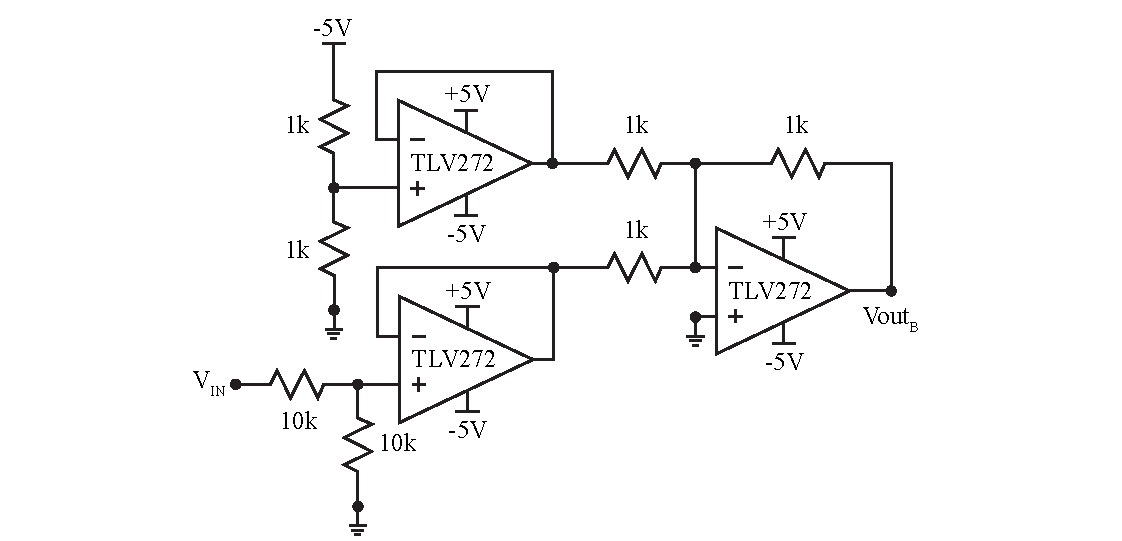
\includegraphics[width=1\textwidth]{Lab6fullshift.pdf}
	\caption{A DC level shifter configured to convert the full range of +/-5 to +5/0.} \label{fig:6fullshift}
\end{figure}

\newpage

%%%%%%%%%%%%%%%%%%%%%%%%%%%%%%%%%%%%%%%%%%%%%%%%%%%%%%%%%%%%%%%%%%%%%%%%%%%%%%%%%%%%%%%%%%%%%%%%%%%%%%%
\subsection{Differential to Single Ended Conversion} \label{ssec:6diff2single}
%%%%%%%%%%%%%%%%%%%%%%%%%%%%%%%%%%%%%%%%%%%%%%%%%%%%%%%%%%%%%%%%%%%%%%%%%%%%%%%%%%%%%%%%%%%%%%%%%%%%%%%

Differential signals, two signals where one signal is 180 degrees out of phase with the other signal, have a variety of applications. The primary benefit of differential signals is increased noise performance but at the cost of extra hardware, you need two of everything. Converting from a differential signal to a singled ended signal can be accomplished fairly simply with a difference amplifier. 

\begin{figure} [h]
	\centering
		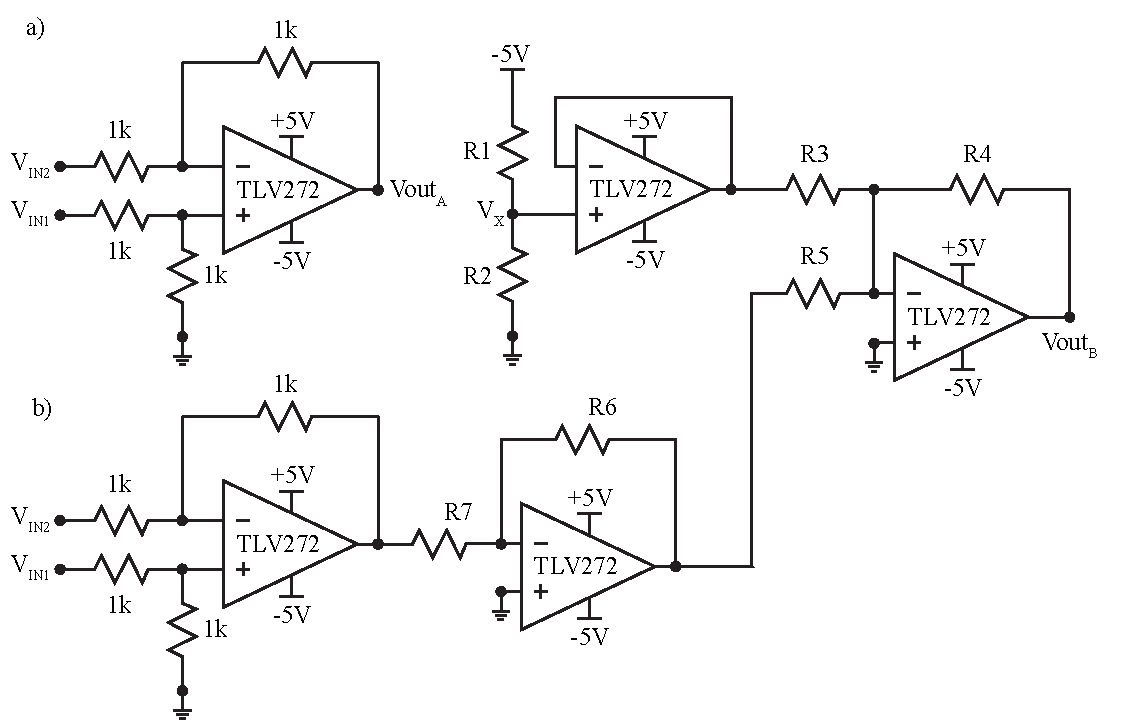
\includegraphics[width=1\textwidth]{Lab6difftosingle.pdf}
	\caption{A difference amplifier that converts a differential signal to single ended (a) and a combination of the level shifter and differential to single ended converter (b).} \label{fig:6difftosingle}
\end{figure}

\begin{enumerate}
	\item Simulate the circuit in \hyperref[fig:6difftosingle]{Figure \ref*{fig:6difftosingle} (a)} using a transient analysis with a stop time of 1m (.tran 1m). Set $V_{IN1}$ to a sine wave with a 0 V DC offset, 0.5 V amplitude, and a 1k Hz frequency. Set $V_{IN2}$ to a sine wave with a 0 V DC offset, 0.5 V amplitude, a 1k Hz frequency, and a phase of 180 degrees. Save an image of the circuit and a plot of the input (both inputs) and output voltages for submission to Canvas. \label{itm:6ssec3itm1}
	\item Determine the resistor values for R1 through R7, recall that there are limited quantities in the lab kit. Choose R1 and R2 so that $V_X$ is 2.5V, R3, R4, and R5 so that both voltages are added equally, and R6 and R7 so that the output, $Vout_B$ utilizes as much of the full range, 0 to 5V, as possible without clipping. \label{itm:6ssec3itm2}
	\item Simulate the circuit in \hyperref[fig:6difftosingle]{Figure \ref*{fig:6difftosingle} (b)} using a transient analysis with a stop time of 1m (.tran 1m). Set $V_{S1}$ and $V_{S2}$ to their previously defined values. Save an image of the circuit and a plot of the input (both inputs) and output voltages for submission to Canvas. \label{itm:6ssec3itm3}
	\item Explain how the circuit in \hyperref[fig:6difftosingle]{Figure \ref*{fig:6difftosingle} (b)} works  in a few sentences. Submit your answer as part of the document submitted to Canvas. \label{itm:6ssec3itm4}
\end{enumerate}

\newpage

%%%%%%%%%%%%%%%%%%%%%%%%%%%%%%%%%%%%%%%%%%%%%%%%%%%%%%%%%%%%%%%%%%%%%%%%%%%%%%%%%%%%%%%%%%%%%%%%%%%%%%%
\section{In-Lab Requirements}
%%%%%%%%%%%%%%%%%%%%%%%%%%%%%%%%%%%%%%%%%%%%%%%%%%%%%%%%%%%%%%%%%%%%%%%%%%%%%%%%%%%%%%%%%%%%%%%%%%%%%%%

The following must be completed at the start of lab. 

\begin{enumerate}
	\item \hyperref[ssec:6buff]{Section \ref*{ssec:6buff}}
		\begin{enumerate}
			\item \hyperref[itm:6ssec1itm1]{Item \ref*{itm:6ssec1itm1}}: Image of the circuit and a table of output voltages.
			\item \hyperref[itm:6ssec1itm2]{Item \ref*{itm:6ssec1itm2}}: Answer to question.
		\end{enumerate}
	\item \hyperref[ssec:6lvlshift]{Section \ref*{ssec:6lvlshift}}
		\begin{enumerate}
			\item \hyperref[itm:6ssec2itm1]{Item \ref*{itm:6ssec2itm1}}: Image of the circuit and a plot of the input and output voltages.
			\item \hyperref[itm:6ssec2itm2]{Item \ref*{itm:6ssec2itm2}}: Answer to question.
			\item \hyperref[itm:6ssec2itm3]{Item \ref*{itm:6ssec2itm3}}: Image of the circuit and a plot of the input and output voltages.
			\item \hyperref[itm:6ssec2itm4]{Item \ref*{itm:6ssec2itm4}}: Plot of the input and output voltages and a circuit demonstration.
			\item \hyperref[itm:6ssec2itm4]{Item \ref*{itm:6ssec2itm5}}: Image of the circuit and a plot of the input and output voltages.
		\end{enumerate}
	\item \hyperref[ssec:6diff2single]{Section \ref*{ssec:6diff2single}}
		\begin{enumerate}
			\item \hyperref[itm:6ssec3itm1]{Item \ref*{itm:6ssec3itm1}}: Image of the circuit and a plot of the input and output voltages.
			\item \hyperref[itm:6ssec3itm3]{Item \ref*{itm:6ssec3itm3}}: Image of the circuit and a plot of the input and output voltages.
			\item \hyperref[itm:6ssec3itm4]{Item \ref*{itm:6ssec3itm4}}: Answer to question.
		\end{enumerate}
\end{enumerate}

Complete the following in lab.

%%%%%%%%%%%%%%%%%%%%%%%%%%%%%%%%%%%%%%%%%%%%%%%%%%%%%%%%%%%%%%%%%%%%%%%%%%%%%%%%%%%%%%%%%%%%%%%%%%%%%%%
\subsection{Construction} \label{ssec:6const}
%%%%%%%%%%%%%%%%%%%%%%%%%%%%%%%%%%%%%%%%%%%%%%%%%%%%%%%%%%%%%%%%%%%%%%%%%%%%%%%%%%%%%%%%%%%%%%%%%%%%%%%

\begin{enumerate}
	\item Construct the circuit from \hyperref[itm:6ssec2itm5]{Section \ref*{ssec:6lvlshift} Item \ref*{itm:6ssec2itm5}}. Set Wavegen1, $V_{IN}$, to a sine wave with a 5 V amplitude, 0 V offset, and a frequency of 1 kHz. \label{itm:6ssec4itm1}
	\item Plot the input and output voltages, save an image of the plot. \label{itm:6ssec4itm2}
	\item Construct the circuit from \hyperref[itm:6ssec3itm3]{Section \ref*{ssec:6diff2single} Item \ref*{itm:6ssec3itm3}}. Set Wavegen1 to $V_{IN1}$ and Wavegen2 to $V_{IN2}$. \label{itm:6ssec4itm3} Synchronize wavegen1 and wavegen2 using the dropdown in the wavegen tab of waveforms. It is located two tabs to the right of "Run all" and is defaulted to "No synchronization".
	\item Plot the input (differential) and the output voltages, save an image of the plot. \label{itm:6ssec4itm4}
\end{enumerate}



%%%%%%%%%%%%%%%%%%%%%%%%%%%%%%%%%%%%%%%%%%%%%%%%%%%%%%%%%%%%%%%%%%%%%%%%%%%%%%%%%%%%%%%%%%%%%%%%%%%%%%%
\section{Write Up}
%%%%%%%%%%%%%%%%%%%%%%%%%%%%%%%%%%%%%%%%%%%%%%%%%%%%%%%%%%%%%%%%%%%%%%%%%%%%%%%%%%%%%%%%%%%%%%%%%%%%%%%

Include the following in the write up.

\begin{enumerate}
	\item \hyperref[ssec:6const]{Section \ref*{ssec:6const}}
		\begin{enumerate}
			\item \hyperref[itm:6ssec4itm1]{Item \ref*{itm:6ssec4itm1}}: Schematic of the circuit, do not copy the schematic from the lab manual, an image from LTspice is fine. 
			\item \hyperref[itm:6ssec4itm2]{Item \ref*{itm:6ssec4itm2}}: Plot of the input and output voltages. 
			\item \hyperref[itm:6ssec4itm1]{Item \ref*{itm:6ssec4itm3}}: Schematic of the circuit, do not copy the schematic from the lab manual, an image from LTspice is fine. 
			\item \hyperref[itm:6ssec4itm2]{Item \ref*{itm:6ssec4itm4}}: Plot of the input and output voltages. 
		\end{enumerate}
\end{enumerate}

Discuss the two circuits constructed in lab. Explain how each circuit works at the block level and how resistor tolerance could or could not have an effect on the output. Also explain the design choices for the circuit, \hyperref[itm:6ssec3itm3]{Section \ref*{ssec:6diff2single} Item \ref*{itm:6ssec3itm3}}, constructed in lab. Which resistors were chosen and why? 
